\chapter{An Incomplete Theory}
\label{sec:theo}

One of the great questions that humans have always tried to answer is
what are the fundamental building blocks of the universe and what are the rules that govern them?
Attempts at answering this question have ranged from
philosophical approach of \textit{`atomism'} by the ancient Greeks \cite{theo-atomism}
to the discovery of atomic structure by Ernest Rutherford \cite{theo-rutherford}.

The the current best answer to this question is the \textit{`Standard Model'},
a mathematical description of a finite set of fundamental particles and their interactions.
%The Standard Model's abilty to describe data is formidable
%and as such it is the foundation of the field of particle physics 
However, it is known that this is not a complete theory and there must be
a deeper underlying theory that lies beyond the Standard Model.

This chapter firstly aims to describe the Standard Model and its key predicitions
with respect to the analyses within the context of this thesis.
Section~\ref{theo-sm} briefly describes the Standard Model and
Section~\ref{theo-qcd} describes QCD and jet formation,
and Section~\ref{theo-pdf} describes the theoretical understanding
of the structure of the proton, known as the parton density function.

Finally, Section~\ref{theo-bsm} will discuss physics Beyond the Standard Model (BSM);
specifically why it is thought that BSM physics is needed
and what are some of the possible models that one can search for.

\section{The Standard Model}
\label{theo-sm}

The Standard Model is a quantum field theory,
which combines the electroweak theory~\cite{theo-glashow},
Quantum Chromodynamics (QCD)~\cite{theo-qcd},
and the Brout-Englert-Higgs mechanism~\cite{theo-be,theo-higgs}.

The Standard Model is made up of 18 fundamental particles,
which means that they are not composed of other consituent particles,
and describes the interactions between them in 4 forces.

\subsection{Particles}

The fundamental particles of the Standard Model
are grouped into three families of particles with similar properties;
known as quarks, leptons and bosons.

\begin{itemize}[leftmargin=*]
\item\textbf{Quarks:}
  Quarks are fermions, meaning they are spin-$\frac{1}{2}$ particles,
  that iteract with the strong force, which is described below.
  There are 6 different types of quarks, known as flavours, arranged in 3 generations.
  Table~\ref{tab:theo-sm_quarks} summarises the flavours of quark and their key properties,
  the values are taken from~\cite{obj-bjets_PDG}.
  For each quark there is also an anti-quark, which has identical mass and spin, but opposite charge and quantum numbers.
  %\end{itemize}
  {\renewcommand{\arraystretch}{1.5}
  \begin{table}[!ht]
  \begin{center}
    \begin{tabular}{|c||c|c|c|c|}
      \hline
    Quark Flavour & Symbol & Charge            &  Spin           &  Mass [GeV]\\
    \hline
    Up            &   $u$  &  $+\frac{2}{3}$   &  $\frac{1}{2}$  &  0.02\\
    Down          &   $d$  &  $-\frac{1}{3}$   &  $\frac{1}{2}$  &  0.05\\
    \hline                                                   
    Charm         &   $c$  &  $+\frac{2}{3}$   &  $\frac{1}{2}$  &  1.3 \\
    Strange       &   $s$  &  $-\frac{1}{3}$   &  $\frac{1}{2}$  &  0.1 \\
    \hline                                                      
    Top           &   $t$  &  $+\frac{2}{3}$   &  $\frac{1}{2}$  &  173  \\
    Bottom        &   $b$  &  $-\frac{1}{3}$   &  $\frac{1}{2}$  &  4.2  \\
    \hline  
  \end{tabular}
    \caption{The key properties of the 6 flavours of quark in the Standard Model,
    organised into the three generations of quarks.}
  \label{tab:theo-sm_quarks}
  \end{center}
  \end{table}}

\item\textbf{Leptons:}
  Leptons are fermions that, unlike the quarks, do not interact with the strong force
  There are 6 different types of leptons,
  arranged into  3 generations, each containing a charge $-1$ particle and a charge 0 neutrino.
  Table~\ref{tab:theo-sm_leptons} summarises the leptons and their key properties.
  The mass of the neutrino is not well known, but it is known to be non-zero and the sum of the three is less than a few eV ~\cite{theo-nu_mass}.
  As for quarks, for each lepton there is also an anti-lepton.
\newpage
  {\renewcommand{\arraystretch}{1.5}
  \begin{table}[!ht]
  \begin{center}
    \begin{tabular}{|c||c|c|c|c|}
      \hline
    Lepton            & Symbol        & Charge  &  Spin           &  Mass [GeV]\\
    \hline
    Electron          &   $e$         &  -1    &  $\frac{1}{2}$   &  \num{5.1e-4}\\
    Electron Neutrino &   $\nu_e$     &  0     &  $\frac{1}{2}$   &  -\\
    \hline                                   
    Muon              &   $\mu$       &  -1    &  $\frac{1}{2}$   &  0.106 \\
    Muon Neutrino     &   $\nu_{\mu}$  &  0     &  $\frac{1}{2}$   &  -\\
    \hline                                      
    Tau               &   $\tau$       &  -1   &  $\frac{1}{2}$   &  1.8\\
    Tau Neutrino      &   $\nu_{\tau}$  &  0    &  $\frac{1}{2}$   &  -\\
    \hline  
  \end{tabular}
    \caption{The 6 types of lepton in the Standard Model and their key properties,
    organised into the three generations of leptons. Neutrino masses are not well known. }
  \label{tab:theo-sm_leptons}
  \end{center}
  \end{table}}
 
\item\textbf{Bosons:}
  The bosons are the set of spin-0 or spin-1 particles in the Standard Model,
  which act as the mediators of the forces that will be described below.
  Table~\ref{tab:theo-sm_bosons} summarises the bosons and their key properties.
  The bosons are their own anti-particle, with the exception of the $W^{+}$ and $W^{-}$
  which are each others anti-particle.

  {\renewcommand{\arraystretch}{1.5}
  \begin{table}[!ht]
  \begin{center}
    \begin{tabular}{|c||c|c|c|c|}
      \hline
    Boson            & Symbol        & Charge  &  Spin  &  Mass [GeV]\\
    \hline
    Photon           &   $\gamma$    &  0      &  1     &  0 \\
    W-boson          &   $W^{\pm}$    & $\pm$1  &  1     &  80 \\
    Z-boson          &   $Z_0$       &  0      &  1     &  91\\
    Gluon            &   $g$         &  0      &  1     &  0 \\
    Higgs Boson      &   $H$         &  0      &  0     &  125\\
    \hline  
  \end{tabular}
    \caption{The key properties of the bosons of the  Standard Model. }
  \label{tab:theo-sm_bosons}
  \end{center}
  \end{table}}
    
\end{itemize}

\subsection{Forces}

As described above, the Standard Model combines three key theories in a
$SU(3)~\text{x}~SU(2)~\text{x}U(1)$ gauge symmetery,
where each symmetry part describes a force mediated by a boson given above.

The first key theory is electro-weak theory.
The theory describes the mixing of the fields given in the symmetry group $SU(2)~\text{x}~U(1)$,
which arises in three distinct interation types, which are grouped into two forces:
the electro-magnetic and weak forces.

\begin{itemize}[leftmargin=*]
\item\textbf{Electro-Magentic (EM):}

  The EM force is an interaction between charged particles which is mediated by the photon.
  The coupling is proportional to the product of the two charged particles.
  multiplied by the EM coupling constant $\alpha_{EM}$, where $\alpha_{EM} \sim$ 1/137.\vspace{0.5em}

\item\textbf{Weak Force:}

  The weak force is composed of the two remaing interactions from electroweak theory;
  the neutral current interaction and the charged current interaction.
  
  The neutral current interaction is mediated by the $Z_0$ boson, has a universal interaction to all fermions,
  and does not allow for flavour change within the interactions.

  The charged current interaction is mediated by the $W^+$ and $W^-$ boson, has a universal interaction with all fermions,
  and flavour changing interactions are allowed.
  Futhermore, due to the fact that the charged current interactions couples with weak eigenstates of fermions rather than
  their flavour eigenstates, the charged current interaction allows for interactions that change generation of the fermion's flavour.
  
  In the quark sector, the relative amplitudes of each flavour changing interactions is described by the CKM matrix;
  the structure of this matrix supresses generational changing interactions,
  in particular those from the 3rd generation  are highly supressed.
  This feature will be prove important identifying the presence of $b$-quarks at the ATLAS detector.
  Both interactions of the weak force are much weaker than the EM force due to the large masses of the mediating particles
  ($\alpha_{Weak}/\alpha_{EM} \sim 10^{-4}$).\vspace{0.5em}
  
\item\textbf{Strong Force:}

  Quantum chromodynamics (QCD) is a theory described by a SU(3) gauge symmetry that describes the interactions between quarks and gluons.
  The symmetry leads to 3 colour charges, which are red, green and blue,
  where the addition of the three gives a colour neutral object.
  The strong interaction is mediated by the gluon and will interact particles that have colour charge, which are quarks and gluons.
  The fact that the gluon has colour charge means that gluon is self interacting.
  QCD is important in terms of understanding jet formation and the production of the
  largest background in a dijet search, so further detail will follow in section in Section~\ref{theo-qcd}.

\item\textbf{Higgs Mechanism:}
  The Higgs Mechanism \footnote{Also known as the Higgs-Englert-Brout mechanism}
  introduces an extra scalar field to the Standard Model,
  which has a Higgs potential given by the so-called `mexican-hat potential'.
  This allows for spontaneous symmetry breaking which gives mass to the boson of the Standard Model.
  In addition a Yukawa coupling between the scalar field and the fermions gives rise to the mass of fermions
  \footnote{With the exception of the neutrinos, whose mass is not described by the Standard Model}.
  A final prediction of the Higgs mechanism was a further spin-0 boson, known as the Higgs boson.
  The first observation of the Higgs Boson by the ATLAS~\cite{theo-higgs_atlas} and CMS~\cite{theo-higgs_cms} experiments
  in 2012 confirmed the Higgs mechanism and is seen as a great triumph of the Standard Model.
\end{itemize}

\section{QCD: Jet Formation and Dijet Production}
\label{theo-qcd}

As described above Quantum chromodynamics (QCD) is a theory that describes the strong interaction between
quarks and gluons.
QCD therefore describes two elements that are critical to the analysis being presented in this thesis;
specifically the formation of jets and the production of dijet events through QCD in proton-proton collisions,
which will be the dominant background in the analysis.
This section will firstly describe renormalisation of QCD, which is important for understanding how QCD works
and will then describe the process of dijet production in hadron collisions and jet formation.

\subsection{Renormalisation and the Running of $\alpha_S$}

For any calcuation in QCD, or any theory, one must consider the higher order loops to the propagator in;
for example for a simple gluon propagator there are additional first-order loops shown in Figure~\ref{fig:theo-qcd_gluon}.
These additional loops lead to divergences in calculations of scattering events.

\begin{figure}[!hbt]
  \begin{center}
    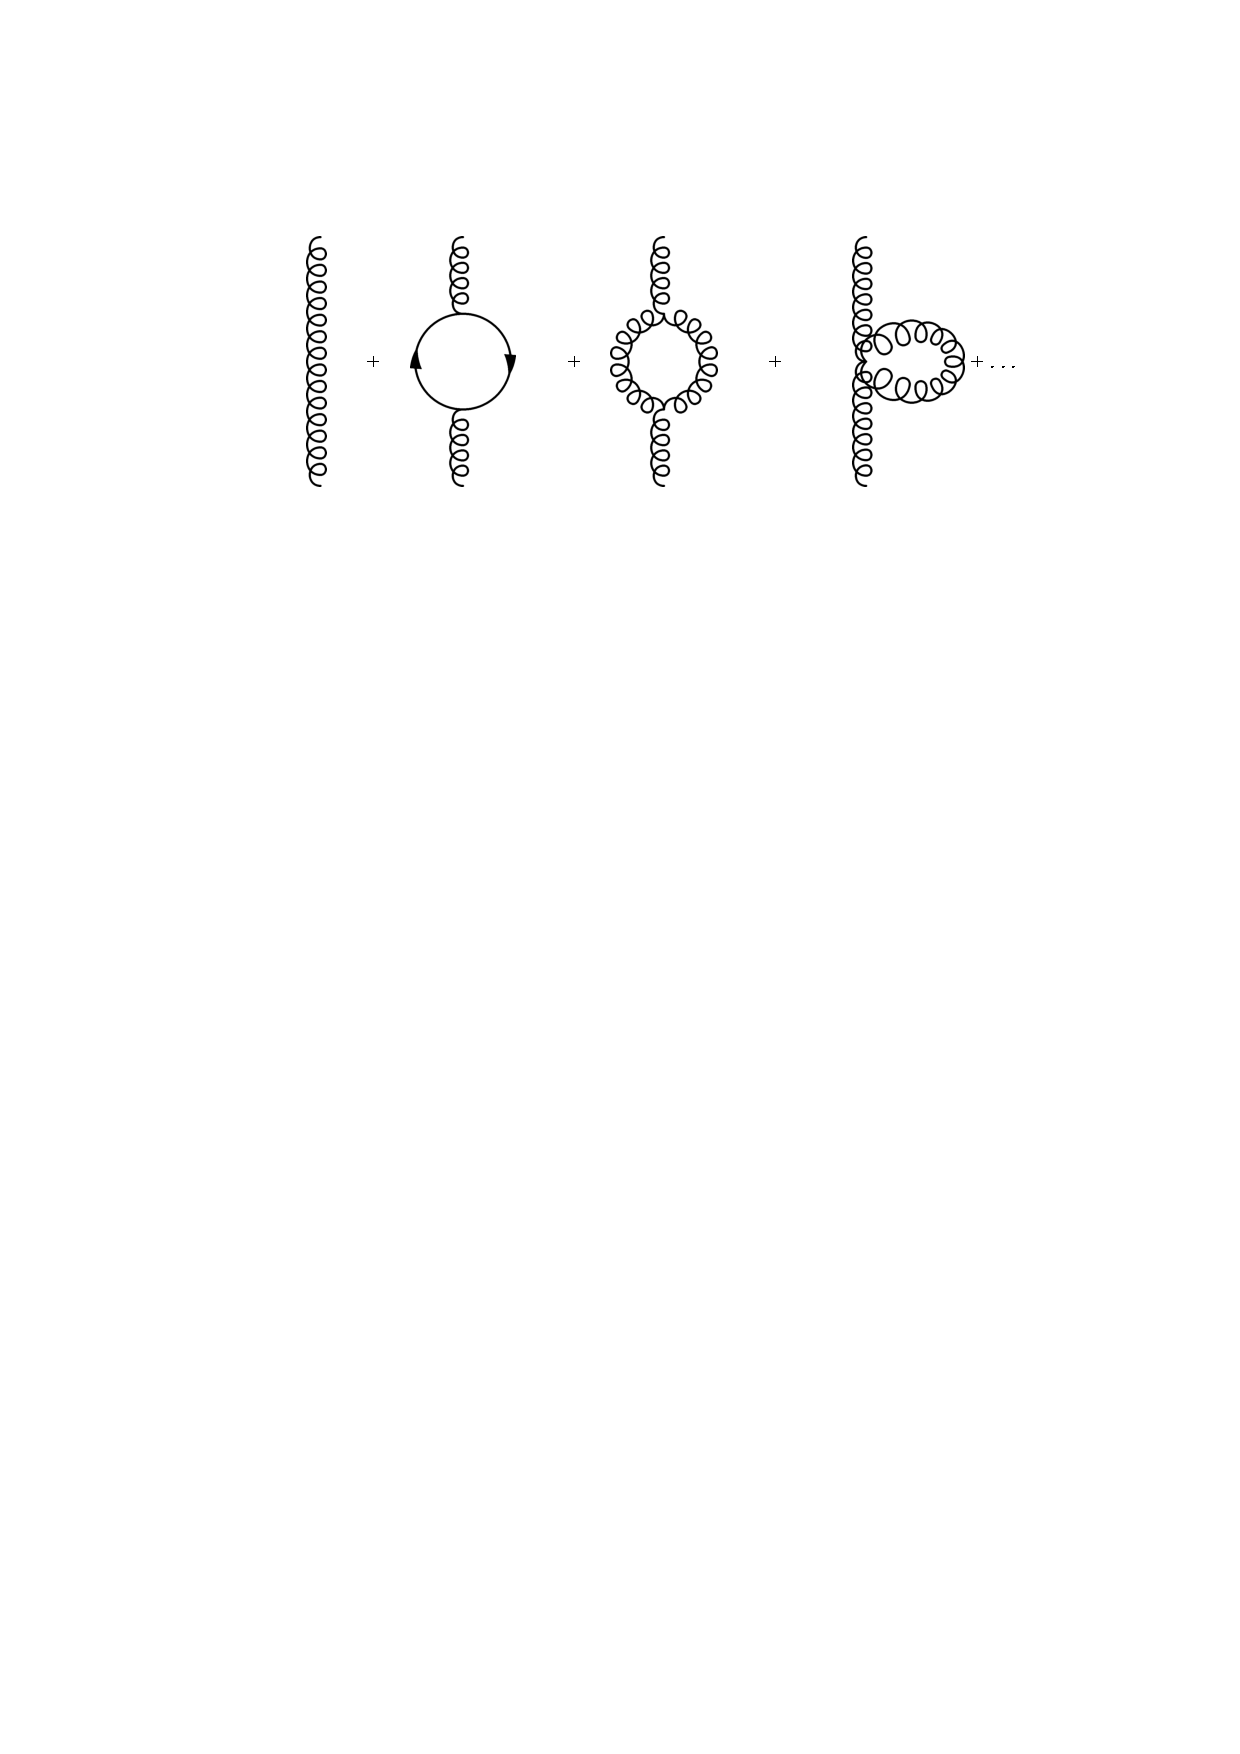
\includegraphics[width=0.7\linewidth, angle=0]{figs/Theory/qcd_gluon_loop.pdf}
  \end{center}
  \caption[A schematic showing the gluon propagator with the additional first order loops.]
  {A schematic showing the gluon propagator with the additional first order loops~\cite{det-thesis_kate}.}
  \label{fig:theo-qcd_gluon}
\end{figure}

To avoid these divergences, there is a well accepted mathematical tool known as renormalisation,
where one effectively rescales the fields in the lagrangian.
This is done such that the divergences are removed
and one can peform calculations of QCD in a pertubative expansion.
This leads to a dependance of the strong coupling, $\alpha_S$ on the renormalisation scaled used, $\mu_R$,
an effect known as the running of $\alpha_S$.
To get an effective strength of the strong interaction in any given process,
$\mu_R$ is set close to the scale of the momentum transfer $Q$ of the process.%$\alpha_S($\mu_R \sim Q^{2}$).
The running of $\alpha_S$ is found in to agree between experimental observation and theory;
Figure~\ref{fig:theo-qcd_running} shows the measured values of
the strong coupling constant, $\alpha_S$ as a function of the energy scale, $Q$, in a range of theories and experiment.

\begin{figure}[!hbt]
  \begin{center}
    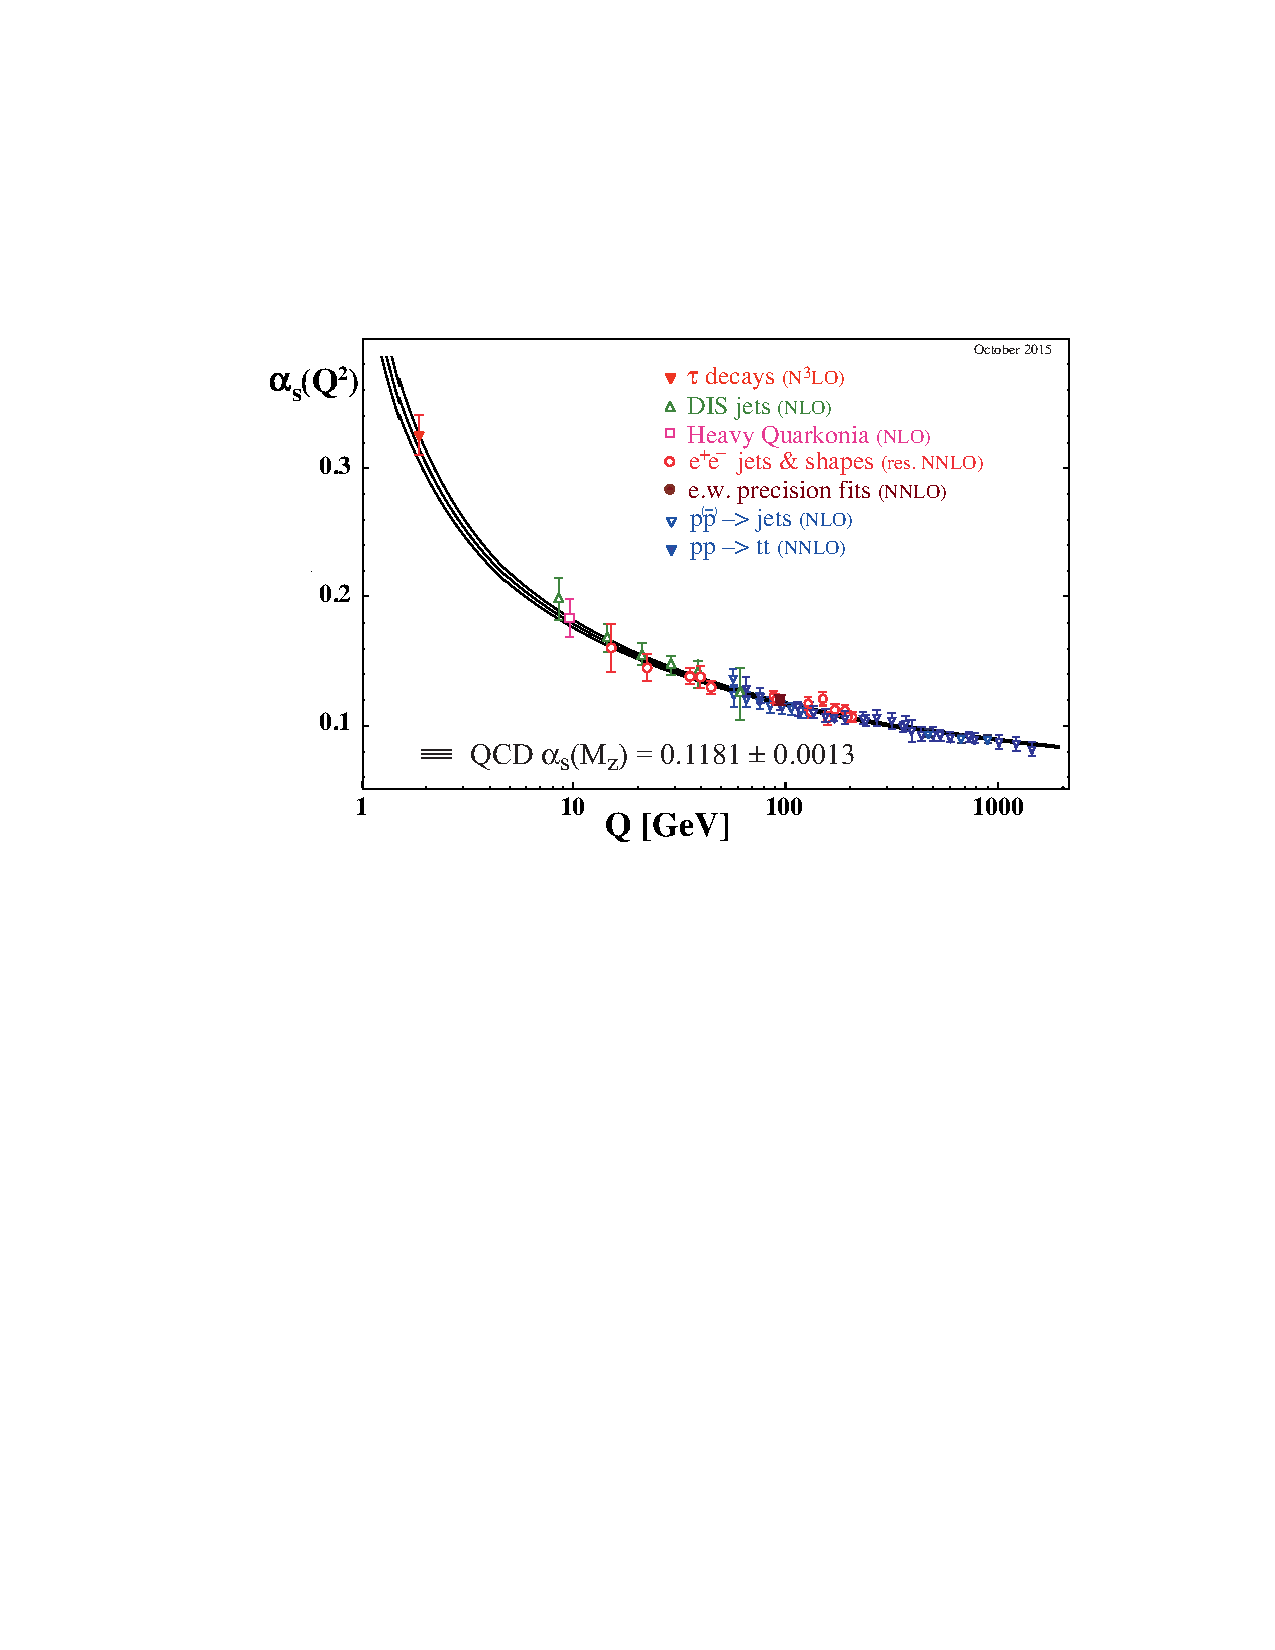
\includegraphics[width=0.7\linewidth, angle=0]{figs/Theory/qcd_running.pdf}
  \end{center}
  \caption[Summary of measurements of $\alpha_S$ as a function of the energy scale $Q$.
    The respective degree of QCD perturbation theory used in the extraction of $\alpha_S$ is indicated in brackets
    (NLO: next-to-leading order; NNLO: next-to-next-to leading order; res. NNLO: NNLO matched with resummed next-to-leading logs; N3LO: next-to-NNLO).]
          {Summary of measurements of $\alpha_S$ as a function of the energy scale $Q$.
            The respective degree of QCD perturbation theory used in the extraction of $\alpha_S$ is indicated in brackets
            (NLO: next-to-leading order; NNLO: next-to-next-to leading order; res. NNLO: NNLO matched with resummed next-to-leading logs; N3LO: next-to-NNLO)~\cite{theo-qcd}.}
  \label{fig:theo-qcd_running}
\end{figure}

\subsection{Multi-jet Production at the LHC}

Dijet production is one of the most common process that occurs in any hadron collider.
Jet formation is described below, so I first want to focus on the dijet production at the parton level;
which is the description of two quarks/gluons from protons interacting through QCD to give
two quarks or gluons in the final state.
Figure~\ref{fig:theo-qcd_dijet_feynman} shows a Feynman diagram of one mode of dijet production in proton-proton collision.

\begin{figure}[!hbt]
  \begin{center}
    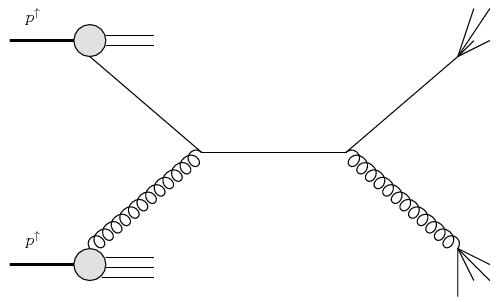
\includegraphics[width=0.7\linewidth, angle=0]{figs/Theory/qcd_dijet_feynman.png}
  \end{center}
%  \caption[Three feynman diagrams illustrating the parton level scatter process in dijet production at the LHC.]
%          {Three feynman diagrams illustrating the parton level scatter process in dijet production at the LHC~\cite{heo-qcd_dijet_feynman}.}
  \caption[A Feynman diagram showing one mode of dijet production at a hadron collider.]
          {A Feynman diagram showing one mode of dijet production at a hadron collider~\cite{heo-qcd_dijet_feynman}.}
  \label{fig:theo-qcd_dijet_feynman}
\end{figure}

To calculate the dijet cross-section, $\sigma$, in a proton-proton collision,
two elements are seperated out in a process called factorisation.
This is formally written as
\begin{equation}
%  \sigma(p_1p_2\to q/g_i q/g_j) = \int dx_1 dx_2 f_1(x_1,\mu^2_F)f_2(x_2\mu^2_F) \sigma(q/g_1,q/g_2, \alpha_s(\mu^2_R),Q^2/\mu^2_F,Q^2/\mu^2_R)
  \sigma = \Sigma_{ij}\int dx_1 dx_2 f_1(x_1,Q^2)f_2(x_2,Q^2) \hat{\sigma}(p_1, p_2\to p_i p_j,Q^2)
\end{equation}
where $f_i$
\subsubsection{Factorisation}
\subsubsection{Hard Scatter}
\subsubsection{Parton Density Functions}


\subsection{Jet Production}

%\subsection{Parton shower}
%\subsection{Hadronisation}

\subsection{A Special Case: $t\bar{t}$}



\section{Beyond the Standard Model}
\label{theo-bsm}

\subsection{Why do we need BSM}
\subsection{Benchmark models}
\subsubsection{Z' Boson}
\subsubsection{Excited b* quark}
